%!TEX root = disclosure_game.tex
\section{Model Description}
\label{app:model_description}

Typically in the UK, a women will have 12 appointments with a midwife during the antenatal period, and in the majority of cases will encounter several different midwives \citep{Redshaw2014} in the course of their care. In the UK, and unlike most healthcare scenarios, maternity notes are held by the patient, so midwives do not have extensive information prior to an appointment unless they have encountered the woman previously. Maternity notes are not generally linked to extra-departmental records, meaning that a history of alcohol related admissions to another service may remain unknown unless revealed by the woman.

According to NICE guidance \citep{NICE2010a,NICE2010} the issue of substance misuse should be raised at the initial booking appointment, followed by subsequent action if a concern is raised is at the discretion of the midwife. This may take the form of specific guidance to reduce intake, or if deemed necessary a referral to a specialist midwife and relevant interdisciplinary team. On alcohol consumption, policy regarding how to determine the level of consumption is at the time of writing generally at the level of local health authority, hospital trust, or according to the best judgement of the individual midwife, with no guidance provided by NICE. This commonly takes the form of average units per week, but may include \ac{T-ACE}\footnote{The \ac{T-ACE} is a four question screening test for alcohol misuse intended specifically for use with pregnant women.} \citep{Sokol1989863} and similar measures. 

Beyond the \enquote{booking} appointment, the onus is on women to raise concerns about their drinking behaviour, or the midwife to probe further if they feel it is warranted. In either case, once a concern has been raised the midwife must respond clinically, and inevitably personally, to the information.

In an ideal world, all interactions with healthcare providers would be immediately and fully disclosive, with no repercussions for the patient. However, alcohol misuse by women is known to attract stigma \citep{Gomberg1988}, and is a recognised barrier to appropriate treatment in the maternity context \citep{NICE2010,Radcliffe2011}.

\subsection{Disclosure Game}
\label{sub:the_game}
%Outline how the scenario translates into a game.
%Brief mention of the game theoretic solution


In order to translate the scenario sketched above into a more abstract, tractable form, we can treat it as a game. A game, in the game theoretic sense, this can be any interaction where the result for one person is dependent on the actions of another. In this scenario, the result for the woman would seem dependent on whether the midwife chooses to refer them for specialist support (although naturally the reality can only be thought of in terms of risk mitigation), and conversely, the right choice for the midwife is somewhat contingent on what the woman is willing to tell them.

A very simple way to represent this would be a game with two players, who both have two possible moves - ask for help, or not; and refer, or not (fig \ref{fig:simplest_game}). Since both parties are invested in the outcome of the pregnancy, we might allow them to share the same payoff if everything ends well. The only time things in this very restricted world obviously end poorly, is if the woman asks for help but does not get any. This implies that a rational player would always refer if asked for help, and is indifferent otherwise - in other words, there are three possible Nash equilibriums.


\begin{figure}[H]
\begin{adjustbox}{center}
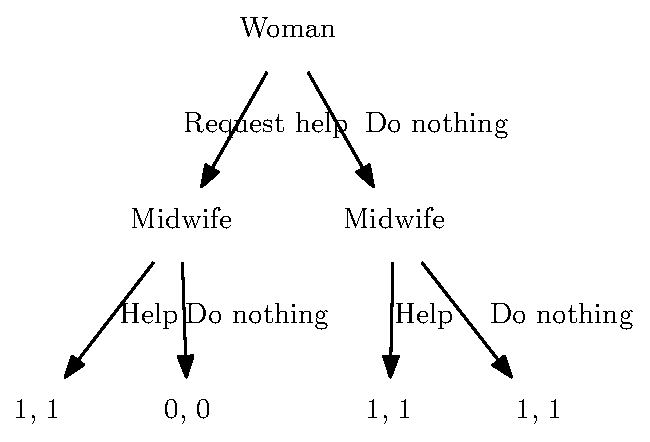
\includegraphics[width=119mm]{figures/simplest_game}
\end{adjustbox}
\caption{A very simple two player game.}

\label{fig:simplest_game}
\end{figure}

The first complication, is that there should be differentiation between referring, and doing nothing because specialist treatment incurs a cost. We can modify the payoffs to reflect this, by reducing the midwife's payoffs when they refer. If the cost of referring is less than the value of a good outcome, then the effect of this is to make the only rational choice when not asked for help is to do nothing.

This simple game is, however not very informative and clearly neglects much of the nuance of the scenario. The wider difficulty here is that the real outcome depends on an attribute of one of the players, rather than their moves. In this case, we would expect the right choices to depend on the alcohol consumption of the woman, rather than entirely on what they have claimed about it.
To reflect this, we would need different variations on the same game to reflect this attribute. 

To resolve this, we can do exactly that, and cast it as a signalling game. We make the simplifying assumption that a woman may have one of only three drinking patterns - light\footnote{Or abstinent, the extent of alcohol consumption being such that it would generally be felt to pose essentially no risk.}, moderate, or heavy. Each of these types of player, will play a different game. This also introduces a third player, who we will call nature. Nature takes the first move, and decides the type of the woman according to some probability distribution; in this case we will allow the probability of types to be uniform. 
This changes the dynamics of play substantially, since the midwife can no longer be certain of which game they are playing, and hence which move yields the best outcome. We must also amend the moves, and payoffs slightly. The woman now claims to be one of the types, and may send a signal to say, for example, that they are a heavy drinker. We will also modify the common payoffs to allow light drinkers to get the best outcome no matter what, and moderate and heavy types to get the best outcome only if referred. We can also differentiate between the consequences of not getting help for these types by letting heavy drinkers have a very negative outcome, and moderate drinkers a slight one (fig \ref{fig:less_simple}).

\begin{figure}[H]
\begin{adjustbox}{center}
\includegraphics[width=119mm]{figures/less_simple_game}
\end{adjustbox}
\caption{A less simple two player game.}

\label{fig:less_simple}
\end{figure}


Correspondingly, they are limited in what signals they may send when claiming to be one of these three types. 

Midwives are treated in a similar fashion, where their type corresponds to how negatively they regard a drinking pattern - non-judgemental, moderately judgemental, and harshly judgemental. The expression of this judgement is not a matter of choice on their part, and is assumed to have no impact on their clinical response, which is to either refer the woman for specialist treatment, or do nothing.

At the end of a game, each player receives a payoff dependent on the actions and types of both players. Because both women and midwives have an interest in the outcome of the pregnancy, and would prefer a healthy baby, the payoff has a common interest component. Hence, both players receive a payoff based on the outcome of pregnancy, but women bear a social cost dependent on the signal they sent and the midwife's reaction to it. Similarly, midwives pay a cost if they refer to a specialist, mirroring the organisational cost of non-routine care. Table \ref{tab:Payoff-matrix} shows the three payoff matrices which together describe the game.



Taken together, this leads to a game tree that is relatively complex (figure \ref{fig:simple_tree} shows a simplified representation, with a detailed view of one branch in figure \ref{fig:zoom_tree}) even at the subgame level. 

As an example, consider the challenge faced by an agent of the heavy drinking type. In order to get the best health outcome, they must be referred and would ideally achieve this without paying any social cost at all. The best move depends on the type, and beliefs of the midwife. For example, a particularly unlucky scenario might be for the midwife to not only be of a harshly judgemental disposition, but to believe that no women really need to be referred. Even a relatively weak belief in this possibility can make the honest signal look like an unwarranted risk.

Rather than attempt to solve for equilibria, agents treat this two player game as taking place against nature, along the lines of adversarial risk analysis \citep{RiosInsua2009}. This effectively translates the game to a pair of decision problems (figure \ref{fig:decision_problems}), which agents attempt to resolve at each turn using a simple decision rule, given their prior beliefs and experience of play.

\begin{figure}[H]
\begin{adjustbox}{center}
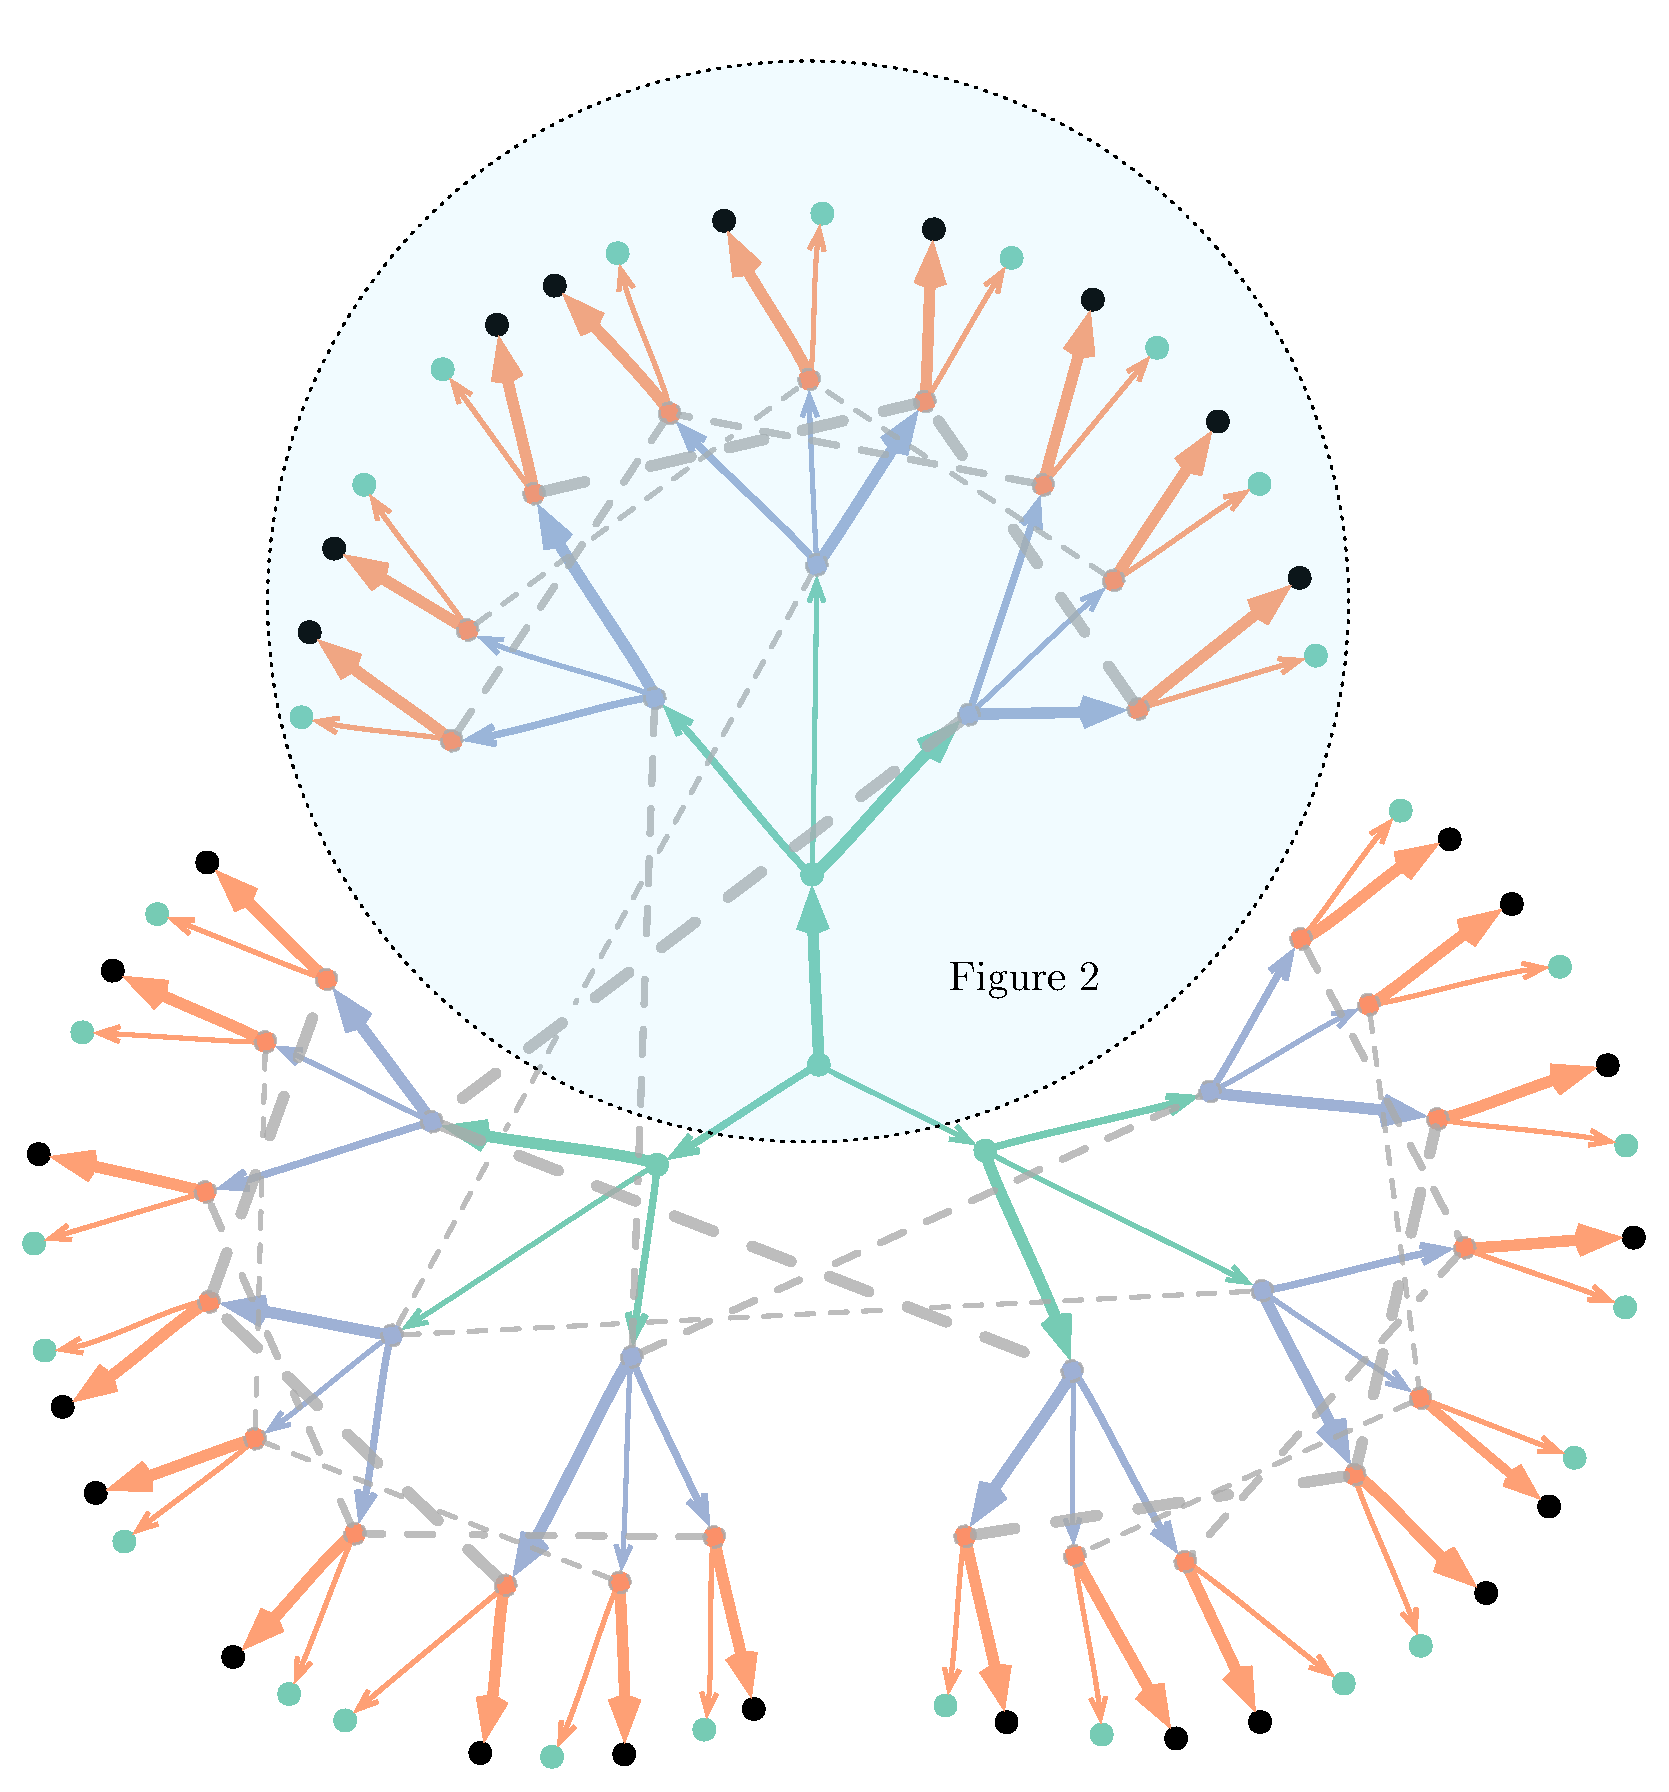
\includegraphics[width=119mm]{figures/rounded_clover_infosets}
\end{adjustbox}
\caption{Simplified game tree. Arrows correspond to two moves by nature, followed by women, and midwives respectively. Line weight distinguishes between information sets, and possible moves, corresponding to ascending player types. For midwives, referral is shown by a heavier arrow. Light terminal nodes indicate that the game may repeat from that point, and black nodes are exits}

\label{fig:simple_tree}
\end{figure}

\begin{figure}[H]
\begin{adjustbox}{center}
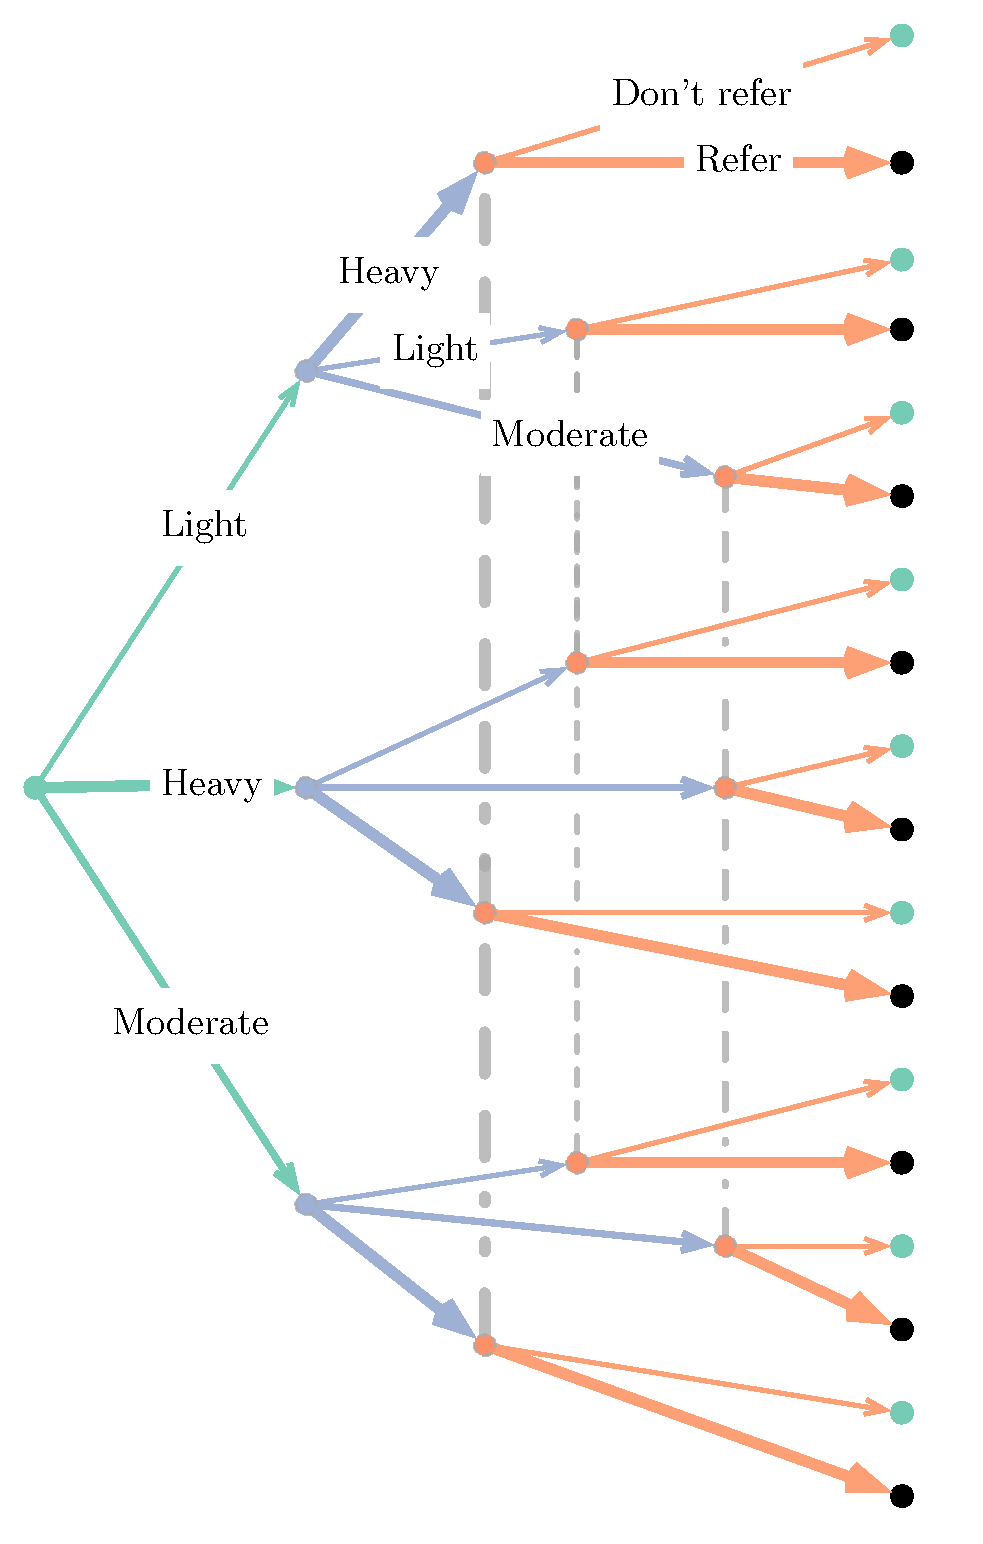
\includegraphics[width=119mm]{figures/tree_zoom}
\end{adjustbox}
\caption{Detail view of a single game tree branch, showing the possible moves by each player, with information sets for midwives}

\label{fig:zoom_tree}
\end{figure}

\begin{figure}[H]
\centering
\subfloat[Women (heavy drinkers)]{\includegraphics[width=119mm]{figures/women_influence}}
\vskip\baselineskip
\subfloat[Midwives]{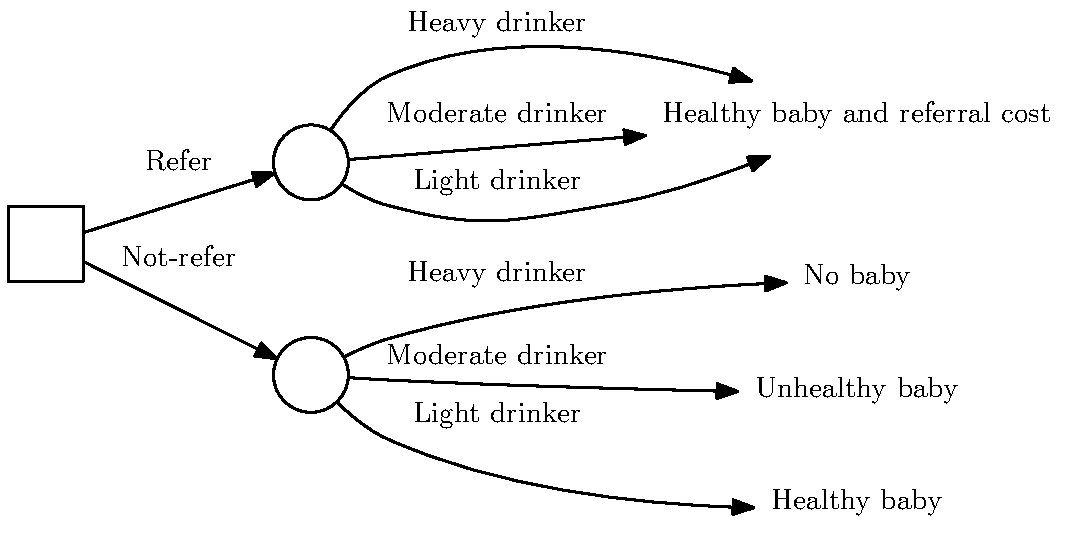
\includegraphics[width=119mm]{figures/mw_influence}}
\caption{Influence diagrams, showing the game broken into two decision problems. Squares indicate a decision node, while circles are (from the perspective of the agent) chance nodes}

\label{fig:decision_problems}
\end{figure}

%Might belong in a more methody bit? Read some stuff to check..
To formally define the game, let \(N = \{m, w\}\) be the set of players each with a private type \(\theta_{i} \in \Theta\), and a set of types \(\Theta=\{l, m, h\}\), with pure strategies \(A_{m}=\{r,n\}, A_{w}=\{l, m, h\}\). Here, \(\{l, m, h\}\) correspond to light, moderate, and heavy alcohol consumption for women, and non-judgemental, moderately judgemental, and harshly judgemental for midwives. Midwives' pure strategies \(\{r,n\}\) are to refer, or do nothing, and those for women are to signal that they have one of the possible drinking patterns.
Additionally define two utility functions - 
\begin{equation}
u_{w}(s_{w}, s_{m}, \theta_{w}, \theta_{m})=X_{s, s_{w}, \theta_{m}} + X_{h, \theta_{w}, s_{m}}
\end{equation} 
\begin{equation}
u_{m}(s_{w}, s_{m}, \theta_{w})=X_{h, \theta_{w}, s_{m}} + X_{c, \theta_{w}, s_{m}},
\end{equation} with $X_{c}$, $X_{h}$, and $X_{s}$ being the payoff matrices as in table \ref{tab:Payoff-matrix}, $s_{w}$ and $s_{m}$ denoting a specific signal by a woman, and referral response by a midwife. Lastly let \(p_{w}(l, m, h)\), \(p_{m}(l, m, h)\) be distributions over types of women, and midwives respectively.


As noted, rather than solve the game, we allow populations of agents to play it, and hence stipulate further that women are drawn in order from a queue of \(n_{w}\) women (where \(n_{w}=1000\) in all simulations), and play against a midwife chosen at random from a population of \(n_{m}\) (\(n_{m}=100\)). They play for a maximum of \(r_{w}\) rounds (\(r_{w}=12\) following the routine number of ante-natal appointments in the UK \citep{NICE2010a}) or until they are referred, and a new player is drawn from the same distribution that produced the original players to replace them. If they are not referred, they rejoin the back of the queue after their appointment. In either case, they are informed of their payoff after each round and update their beliefs accordingly using one of the rules described in section \ref{sub:the_agents}.

Midwives play for \(r_{m}\) rounds (\(r_{m}=1000\) in all experiments), and conduct appointments in parallel, i.e. if there are 5 midwives, then five women are drawn from the queue and assigned at random to the midwives. 
Unlike women, midwives are only informed of their payoff if they choose to make a referral. Both groups of agents have perfect recall, and midwives are assumed to retrospectively update their observations if they make a referral after a number of appointments.